\documentclass[12pt,a4paper,titlepage]{report}
\usepackage[utf8]{inputenc}
\usepackage[T1]{fontenc}
\usepackage{amsmath}
\usepackage{amsfonts}
\usepackage{amssymb}
\usepackage{graphicx}
\usepackage{changepage} 
\usepackage{systeme}
\usepackage{mathtools}
\usepackage{booktabs}
\usepackage[margin=1in]{geometry}
\usepackage{pdfpages} 

\newcommand\setItemnumber[1]{\setcounter{enumi}{\numexpr#1-1\relax}}
\newcommand{\R}{\mathbb{R}}
\newcommand{\N}{\mathbb{N}}
\newcommand{\C}{\mathbb{C}}
%\setcounter{secnumdepth}{0} 

\date{September 28, 2020}
\title{Math 360 - Project 1: Symbiosis (Mutualism)}
\author{Ethan Rahman}

\begin{document}
	\maketitle
	\tableofcontents
	\pagebreak
	\chapter*{Preface}
	\addcontentsline{toc}{chapter}{Preface}
	This essay was my midterm for my class Math 360: Model Building in Applied Math. I was instructed to write responses to each of the questions in the "Problems" section of this document. Everything in the "Answers" section is what I ultimately turned in. \\
	
	Each of the charts and tables were generated using a Python script. The entire project is available on my github. Including the Python script, the .tex file that generated this document, and a master.sh file. The master.sh file re-runs the entire process from the top to the bottom of my workflow. It runs the Python Script, regenerates the tables and figures, and then re-compiles the LaTeX document in action. 
	\pagebreak
	\chapter*{Problems}
	\addcontentsline{toc}{chapter}{Prompts}
	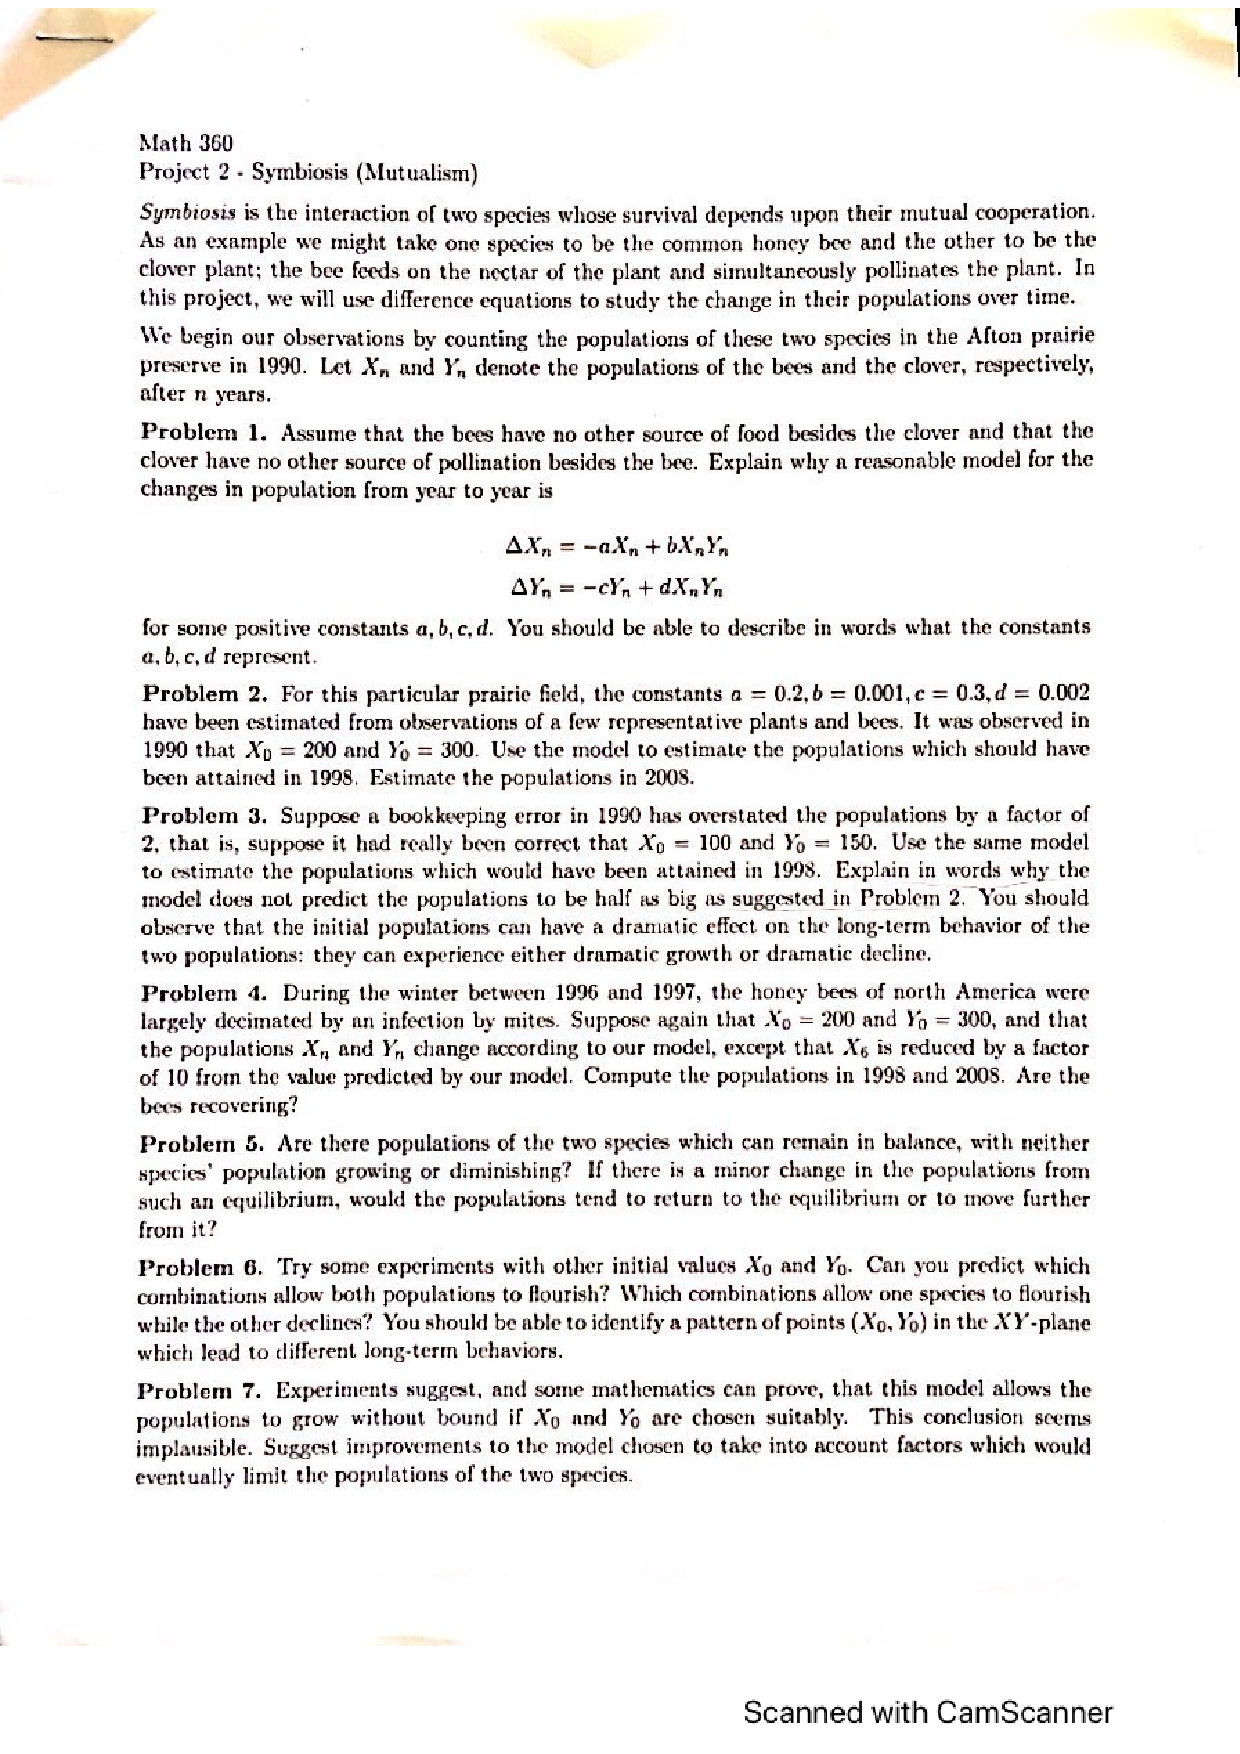
\includepdf[pages=-]{problems.pdf}
	\chapter*{Answers}
	\addcontentsline{toc}{chapter}{Answers}%
	
	\section*{Problem 1}
		%\addcontentsline{toc}{chapter}{\protect\numberline{} Section 1}%
		\addcontentsline{toc}{section}{Problem 1}%
		Honey bees and clover plants have a symbiotic relationship that is mutually beneficial. The assigned problem attempts to model this relationship using a non-linear dynamical system. The model variables are defined in table 1 below.
	
		\begin{table}[ht]
			\centering
			\begin{tabular}{ccccc}
				\toprule
				Variable & Description \\ 
				\midrule 
				\(n\) & Number of years since 1990 \\ 
				\(X_{n}\) & Population of bees at year \(n\) \\
				\(Y_{n}\) & Population of clover plants at year \(n\) \\ 
				\(\Delta X_{n}\) & Net change in bee population during year \(n\) \\
				\(\Delta Y_{n}\) & Net change in clover plant population during year \(n\)   \\ 
				\(a\) & Proportionality constant for death rate of bees \\ 
				\(b\) & Proportionality constant for birth rate of bees  \\ 
				\(c\) & Proportionality constant for death rate of clover plants  \\ 
				\(d\) & Proportionality constant for birth rate of clover plants  \\ 
				\bottomrule
			\end{tabular}
			\caption{Definition of all variables used in this paper.}
		\end{table}
		The exact model is essentially the sum of two terms for each population. The first term in both models can be thought of as the death rate function: \(-aX_{n}\) for bees and \(-cY_{n}\) for clovers. More organisms will die just by random chance or by aging if the population of that organism is higher. The parameters \(a\) and \(c\) represent proportionality constants for the death function in both populations. And because they decrease the population, the sign of the terms are negative. Because bees and clovers have a mutually beneficial relationship we wouldn't expect there to be any interaction effects here. \\
		
		The second term is the birth rate function: \(bX_{n}Y_{n}\) for bees and \(dX_{n}Y_{n}\) for clover plants. Here is where the interaction effects become relevant. Bees benefit from having a higher population of clover plants because they can use feed on more of their nectar. Simultaneously, clover plants benefit from having a higher population of bees because there is a greater chance each bee will spread more pollen. \(b\) and \(d\) represent proportionality constants for the birth function in both populations. \\
		
		Put together, the model is simply the sum of the death rate function and the birth rate function for each population: 
		\[\Delta X_{n} = -aX_{n} + b X_{n}Y_{n}\]
		\[\Delta Y_{n} = -cY_{n} + d X_{n}Y_{n}\]

	\section*{Problem 2}
	\addcontentsline{toc}{section}{Problem 2}%
		For the next section, we're looking at the model when the parameters in table 2 are specified along with the initial points \(X_{0} = 200\) and \(Y_{0} = 300\). 
		\begin{table}[ht]
			\centering
			\begin{tabular}{cl}
				\toprule
				Parameter & Value \\ 
				\midrule 
				\(a\) & 0.2\\ 
				\(b\) & 0.001 \\
				\(c\) & 0.3  \\ 
				\(d\) & 0.002  \\ 
				\bottomrule
			\end{tabular}
			\caption{Set of values for each parameter}
			\label{params1}
		\end{table}
		The results of the model are recorded in table \ref{tab:p2}. For the year 1998, the population of bees is 7,475 while the population of clovers is 14,360. The population of both organisms quickly grows and becomes too large to calculate using Python by the year 2007! So we are unable to provide an answer for the population in the year 2008 but the long run behavior of the model using this set of parameters is clear. The population becomes infinitely large without reaching an equilibrium. 
		\begin{table} 
			\centering
			\begin{tabular}{lrrrr}
\toprule
{} &      \(X\) &      \(Y\) & \(\Delta X\) & \(\Delta Y\) \\
Year &            &            &              &              \\
\midrule
1990 &  2.000e+02 &  3.000e+02 &    2.000e+01 &    3.000e+01 \\
1991 &  2.200e+02 &  3.300e+02 &    2.860e+01 &    4.620e+01 \\
1992 &  2.486e+02 &  3.762e+02 &    4.380e+01 &    7.419e+01 \\
1993 &  2.924e+02 &  4.504e+02 &    7.321e+01 &    1.283e+02 \\
1994 &  3.656e+02 &  5.787e+02 &    1.384e+02 &    2.495e+02 \\
1995 &  5.041e+02 &  8.282e+02 &    3.167e+02 &    5.865e+02 \\
1996 &  8.207e+02 &  1.415e+03 &    9.969e+02 &    1.898e+03 \\
1997 &  1.818e+03 &  3.312e+03 &    5.657e+03 &    1.105e+04 \\
1998 &  7.475e+03 &  1.436e+04 &    1.058e+05 &    2.104e+05 \\
1999 &  1.133e+05 &  2.247e+05 &    2.544e+07 &    5.086e+07 \\
2000 &  2.555e+07 &  5.108e+07 &    1.305e+12 &    2.611e+12 \\
2001 &  1.305e+12 &  2.611e+12 &    3.408e+21 &    6.816e+21 \\
2002 &  3.408e+21 &  6.816e+21 &    2.323e+40 &    4.646e+40 \\
2003 &  2.323e+40 &  4.646e+40 &    1.079e+78 &    2.158e+78 \\
2004 &  1.079e+78 &  2.158e+78 &   2.329e+153 &   4.659e+153 \\
2005 & 2.329e+153 & 4.659e+153 &   1.085e+304 &   2.170e+304 \\
2006 & 1.085e+304 & 2.170e+304 &          inf &          inf \\
2007 &        inf &        inf &          nan &          nan \\
2008 &        nan &        nan &          nan &          nan \\
\bottomrule
\end{tabular}

			\caption{The model values calculated using a Python script. An overflow error is thrown by the year 2006 for \(\Delta X\) and \(\Delta Y\).}
			\label{tab:p2}
		\end{table}
	\section*{Problem 3}
		\addcontentsline{toc}{section}{Problem 3}%
		For problem 3 we use the same parameters in table \ref{params1} but with initial values \(X_{0} = 100\) and \(Y_{0} = 150\). The results here are much more amenable to a visual representation. Figure \ref{fig:p3} depicts the model as a vector field with the specific path taken by the populations when they start at the given initial values.\\ 
		In 1998, the population of bees declines to 43 and the population of clovers is 42. By 2008 there are only 6 bees and 2 clovers. More specific values for the evolution of the population model are given in table \ref{tab:p3}. Over time it appears that both organisms go extinct. \\
		The model does not result in the populations being cut in half from the populations in table \ref{tab:p2} from problem 2. This is because the model is defined by non-linear difference equations. To illustrate this, set \(X_{n} = 2X_{n}\) and \(Y_{n} = 2Y_{n}\) in the birth functions for bees and clovers:
		\[X_{Birth} = b (2X_{n})(2Y_{n}) = 4bX_{n}Y_{n}\]
		\[Y_{Birth} = d (2X_{n})(2Y_{n}) = 4dX_{n}Y_{n}\]
		As you can see,  doubling the populations results in the birth rate increasing by a factor of 4 for both populations! That is, the birth function has increasing returns to scale and is non-linear. \\
		
		\begin{figure}[htbp]
			\centerline{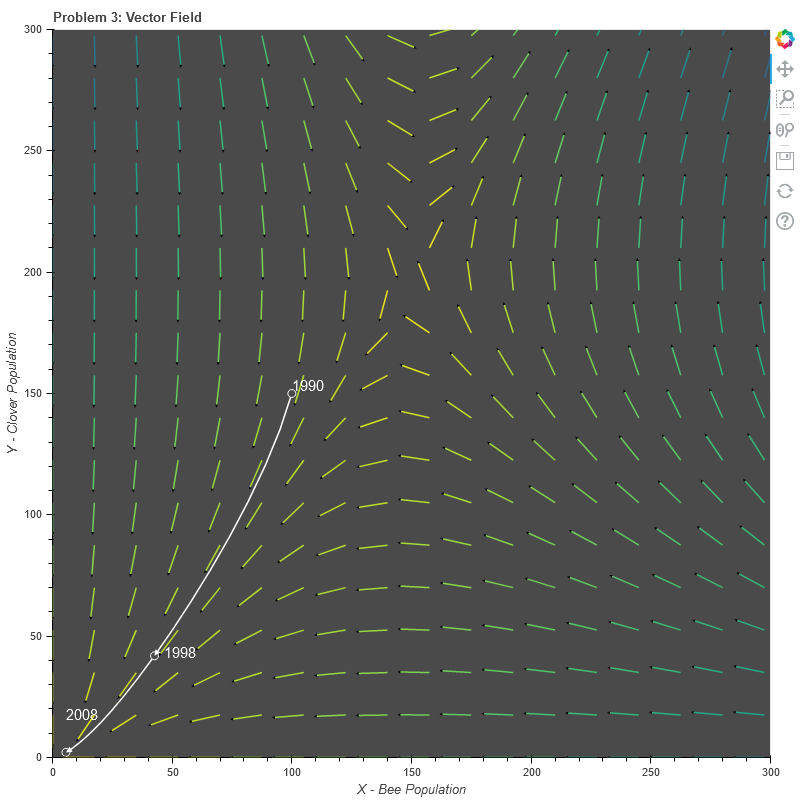
\includegraphics[scale=.5]{charts/problem3_chart.png}}
			\caption{The model is represented as a vector field. The lengths of each vector are kept constant, but the color of each vector is determined by the magnitude of the vector at that point. Light yellow vectors have the lowest magnitude and dark purple vectors have the largest. The white path shows the evolution of the populations when the initial conditions are \(X_{0} = 100\) and \(Y_{0} = 150\) are chosen.}
			\label{fig:p3}
		\end{figure}
		At the same time, the death functions have constant returns to scale:
		\[X_{Death} = -a (2X_{n}) = -2aX_{n}\]
		\[Y_{Death} = -c (2Y_{n}) = -2cY_{n}\]
		As a result, the birth rate tends to increase faster than the death rate as the populations get larger. At the same time however, the death rate will decrease at a slower rate than the birth rate for decreasing populations. If both populations are declining, then generally speaking the death function will stay higher than the birth function in future years. If both populations are increasing, then the birth function will generally be larger than the death function. 
		\begin{table} 
			\centering
			\begin{tabular}{lrrrr}
\toprule
{} &  \(X\) &  \(Y\) & \(\Delta X\) & \(\Delta Y\) \\
Year &        &        &              &              \\
\midrule
1990 & 100.00 & 150.00 &        -5.00 &       -15.00 \\
1991 &  95.00 & 135.00 &        -6.18 &       -14.85 \\
1992 &  88.83 & 120.15 &        -7.09 &       -14.70 \\
1993 &  81.73 & 105.45 &        -7.73 &       -14.40 \\
1994 &  74.00 &  91.05 &        -8.06 &       -13.84 \\
1995 &  65.94 &  77.21 &        -8.10 &       -12.98 \\
1996 &  57.85 &  64.23 &        -7.85 &       -11.84 \\
1997 &  49.99 &  52.39 &        -7.38 &       -10.48 \\
1998 &  42.61 &  41.91 &        -6.74 &        -9.00 \\
1999 &  35.88 &  32.91 &        -5.99 &        -7.51 \\
2000 &  29.88 &  25.40 &        -5.22 &        -6.10 \\
2001 &  24.66 &  19.30 &        -4.46 &        -4.84 \\
2002 &  20.21 &  14.46 &        -3.75 &        -3.75 \\
2003 &  16.46 &  10.71 &        -3.12 &        -2.86 \\
2004 &  13.34 &   7.85 &        -2.56 &        -2.14 \\
2005 &  10.78 &   5.70 &        -2.09 &        -1.59 \\
2006 &   8.68 &   4.11 &        -1.70 &        -1.16 \\
2007 &   6.98 &   2.95 &        -1.38 &        -0.84 \\
2008 &   5.61 &   2.11 &        -1.11 &        -0.61 \\
\bottomrule
\end{tabular}

			\caption{The model evolution for the initial conditions \(X_{0} = 100\) and \(Y_{0} = 150\) given the parameters in table \ref{params1}.}
			\label{tab:p3}
		\end{table}
		This can help explain why small changes in the initial condition of the populations can result in very different long term behaviors - the starting conditions basically determine whether the death function will be larger or smaller than the birth function very early on. And consistent with this description, the vector field in figure \ref{fig:p3} indicates that lower starting populations tend to decline more often than higher starting populations. 
		
	\section*{Problem 4}
		\addcontentsline{toc}{section}{Problem 4}%
		In this problem we have to impose a population shock on the bees in the year 1996 using the initial conditions \(X_{0} = 200\) and \(Y_{0} = 300\). The results of the script are depicted visually in figure \ref{fig:p4} and numerically in table \ref{tab:p3}.
		\begin{figure}[htbp]
			\centerline{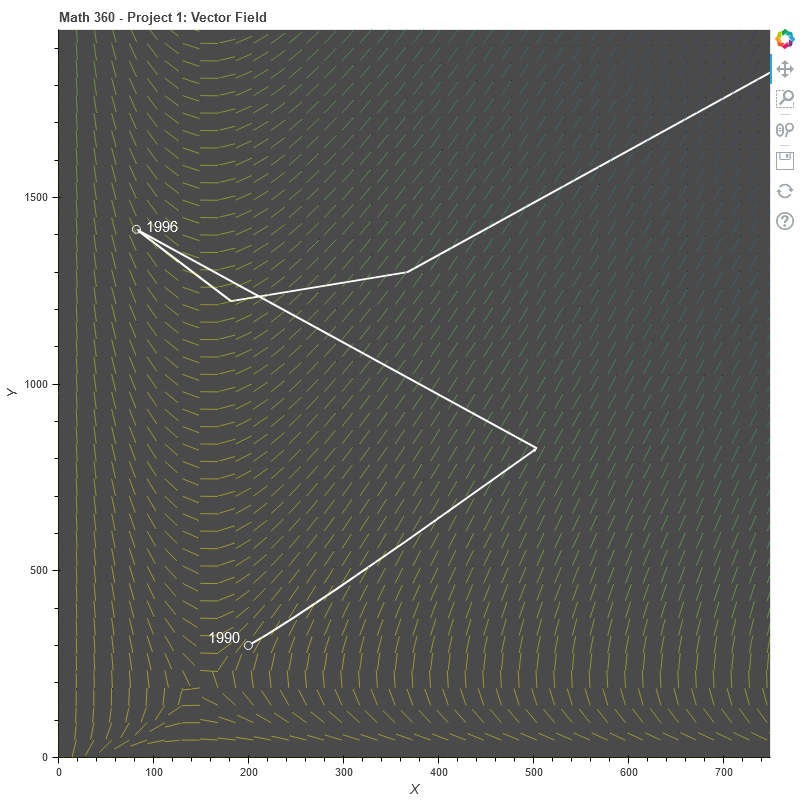
\includegraphics[scale=.5]{charts/problem4_chart.png}}
			\caption{Here the model runs just the same as it did in problem 2 until the year 1996 when the bee population shock is imposed.}
			\label{fig:p4}
		\end{figure}\\
		In 1998 there are only 368 bees, which is much smaller than the 7,475 bee population from problem 2 at the same year. The clover population is 1,300 which is smaller than the original model prediction in problem 2 by more than a factor of 10. But figure \ref{fig:p4} shows that both populations only experience a population decline for a very short period of time. The clover population only declines for one year, and the model never actually gives bees a negative population growth rate outside of the exogenous shock. Both populations quickly recover and by 2008 there are 1.65e+171 bees and 3.31e+171 clover plants. 
	
		\begin{table} 
			\centering
			\begin{tabular}{lrrrr}
\toprule
{} &                                              \(X\) &                                              \(Y\) &                                       \(\Delta X\) &                                       \(\Delta Y\) \\
Year &                                                    &                                                    &                                                    &                                                    \\
\midrule
1990 &                                             200.00 &                                             300.00 &                                              20.00 &                                              30.00 \\
1991 &                                             220.00 &                                             330.00 &                                              28.60 &                                              46.20 \\
1992 &                                             248.60 &                                             376.20 &                                              43.80 &                                              74.19 \\
1993 &                                             292.40 &                                             450.39 &                                              73.21 &                                             128.27 \\
1994 &                                             365.62 &                                             578.66 &                                             138.44 &                                             249.54 \\
1995 &                                             504.06 &                                             828.20 &                                             316.65 &                                             586.47 \\
1996 &                                              82.07 &                                            1414.66 &                                              99.69 &                                            -192.19 \\
1997 &                                             181.76 &                                            1222.47 &                                             185.84 &                                              77.65 \\
1998 &                                             367.60 &                                            1300.12 &                                             404.41 &                                             565.83 \\
1999 &                                             772.02 &                                            1865.95 &                                            1286.14 &                                            2321.30 \\
2000 &                                            2058.15 &                                            4187.24 &                                            8206.36 &                                           15979.80 \\
2001 &                                           10264.51 &                                           20167.05 &                                          204951.98 &                                          407959.65 \\
2002 &                                          215216.49 &                                          428126.69 &                                        92096880.24 &                                       184151409.07 \\
2003 &                                        92312096.73 &                                       184579535.76 &                                  17038905496933.79 &                                  34077792544845.54 \\
2004 &                                  17038997809030.51 &                                  34077977124381.30 &                        580654577555117084508160.00 &                       1161309155106826380902400.00 \\
2005 &                        580654577572156092186624.00 &                       1161309155140904396259328.00 &   674319476909019290268979973228416472480481280.00 &  1348638953818038580537959946456832944960962560.00 \\
2006 &   674319476909019290268979973228416472480481280.00 &  1348638953818038580537959946456832944960962560.00 & 90941351387770685317315676804198526663513477252... & 18188270277554137063463135360839705332702695450... \\
2007 & 90941351387770685317315676804198526663513477252... & 18188270277554137063463135360839705332702695450... & 16540658784467962190888885564475764841016073306... & 33081317568935924381777771128951529682032146612... \\
2008 & 16540658784467962190888885564475764841016073306... & 33081317568935924381777771128951529682032146612... &                                                inf &                                                inf \\
\bottomrule
\end{tabular}

			\caption{The model evolution for the initial conditions \(X_{0} = 200\) and \(Y_{0} = 300\) given the parameters in table \ref{params1} with an exogenous shock in to the bee population in the year 1996. The bee population is reduced by a factor of 10 relative to what was predicted in 1996 in the model from problem 1.}
			\label{tab:p4}
		\end{table}
	
	\section*{Problem 5}
		\addcontentsline{toc}{section}{Problem 5}%
		The most obvious equilibrium that can be seen from the model alone is a trivial equilibrium - when both populations are zero. Nothing changes because both the birth and death terms of the equations are zero. The more interesting question is whether there are non-zero equilibria. By definition, an equilibrium point is when neither population changes. Setting \(\Delta X\) and \(\Delta Y\) equal to zero and solving for \(X_n\) and \(Y_n\)) will yield another equilibrium point. First, solving for \(Y_n\):  
		\[0 = -aX_{n} + b X_{n}Y_{n}\]
		\[a  = b Y_{n}\]
		\[Y_{n} = \frac{a}{b} = \frac{0.2}{0.001} = 200\]
		In order to solve for \(X_n\), the clover equation is needed:
		\[0 = -cY_{n} + d X_{n}Y_{n}\]
		\[c  = d X_{n}\]
		\[X_{n} = \frac{c}{d} = \frac{0.3}{0.002} = 150\]
		Therefore, 150 bees and 200 clover plants should be an equilibrium point for the system. This can be seen visually by looking at a slightly different the vector field in figure \ref{fig:p3}. 
		\begin{figure}[htbp]
			\centerline{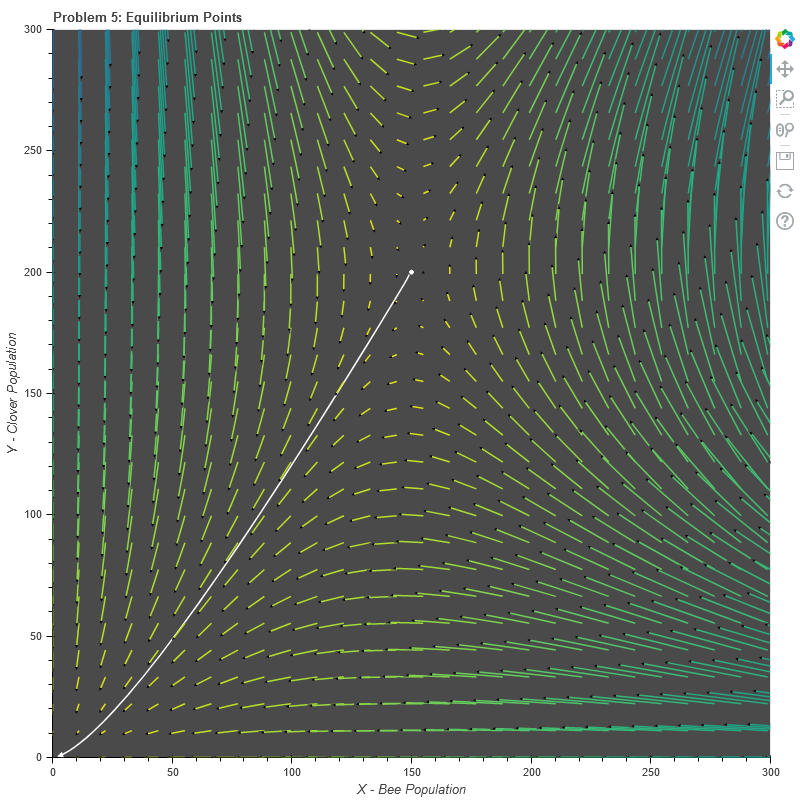
\includegraphics[scale=.5]{charts/problem5_chart.png}}
			\caption{Just as in figure \ref{fig:p3}, the colors correspond to the magnitude of each vector. But in this chart the length also corresponds to magnitude just to make the location of the equilibrium points more clear. The white point at \((150,200)\) denotes the unstable equilibirium point. The white path is the evolution of the model with the initial condition \((149,199)\). Despite starting very close to the equilibrium point, the bees and clovers both eventually die out.}
			\label{fig:p5}
		\end{figure}\\
		In figure \ref{fig:p5}, the two equilibrium points in the model can be seen more clearly.The white point at \((150,200)\) is an unstable equilibrium point. As you approach the white point, the vectors get smaller and smaller, but the vectors never point at the white point directly. Any trajectory not already at \((150,200)\) will veer away either to the origin or grow infinitely large. In contrast, the origin is a stable equilibrium. Many different initial conditions result in landing at the origin as a long term behavior for the model. 
	\section*{Problem 6}
		\addcontentsline{toc}{section}{Problem 6}%
		The most efficient way to get a sense of how different initial conditions affect the long run behavior of the model is to use a visualization such as a histogram coloring. Each point in figure \ref{fig:p6} represents a different initial condition. The point \(100, 100\) is colored purple because the model predicts that both populations will die if they start at that point. The white point is the unstable equilibrium, which is the only place the two animals can remain alive without an unsustainable increase in population or an unsustainable decline in population. 
		\begin{figure}[htbp]
			\centerline{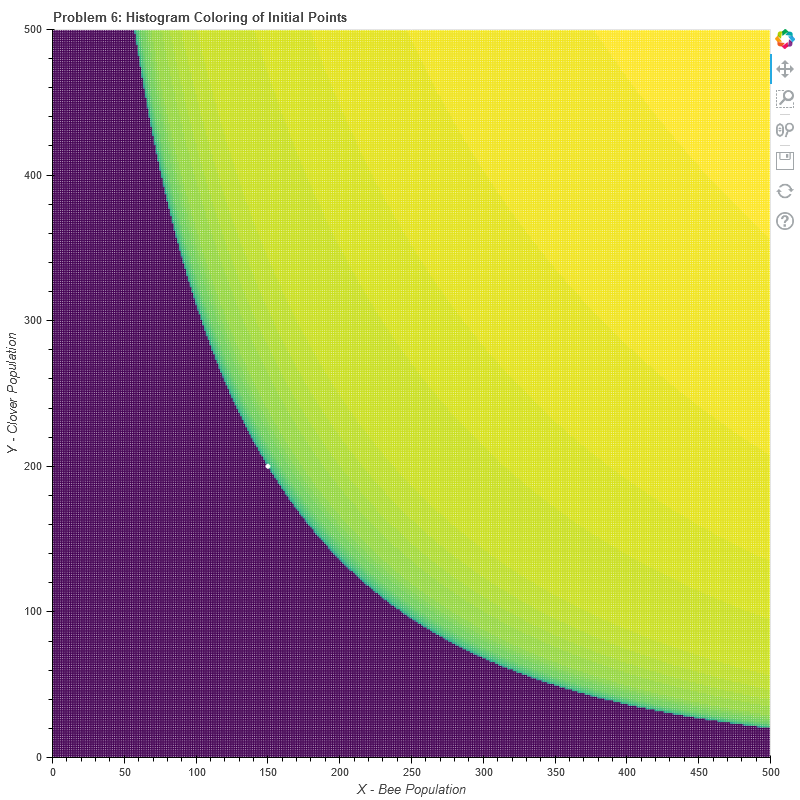
\includegraphics[scale=.5]{charts/problem6_chart.png}}
			\caption{There are three clear regions in the model. If the population of bees and clovers starts in the purple region, they will both eventually go extinct. The white point is the unstable equilibrium point. All the other colors indicate that the populations will grow infinitely large should the bees and clovers start in that region.}
			\label{fig:p6}
		\end{figure}\\
		The regions colored blue, green, and yellow are starting points where the model predicts the populations to grow infinitely large. The colors correspond to how quickly the population blows up. More specifically,the colors are chosen based on the number of iterations of the model it takes before the population exceeds a certain threshold. I choose 10,000 (the threshold is checked for which ever population is larger), but the nice thing about the histogram coloring method is that the coloring doesn't change very much even when the thresholds are changed. 
		
	\section*{Problem 7}
		\addcontentsline{toc}{section}{Problem 7}%
		Several changes to the model can make the model more realistic. First, changing the death rate function to a quadratic function of \(X_n\) is a simple way to avoid having the population of each species grow infinitely. The quadratic function will be insignificant for small populations but then increase very rapidly as the population of each organism gets very large. For instance, its not unreasonable to expect predators to increase their own population in response to the higher population of the animal in question, which would create a mitigating effect that only kicks in for higher populations. \\
		
		The birth functions also need to be adjusted. A big problem here is that the mutualism effects tend to have increasing returns to scale as was explained in the answer to problem 3. This is a very unrealistic assumption in the model. Its far more likely that mutualistic effects have decreasing returns to scale - if the population of bees is too high relative to clovers, the marginal bee added to the population will not be able to pollinate as many clover as the previous bees. The average bee may pollinate a much smaller amount of clovers. Essentially, the birth terms in the model must account for saturation effects. \\
		
		To eliminate increasing returns to scale and also account for saturation, the interaction term is removed from the original birth function and an adjusted interaction term is added. For the clover birth function: 
		\[Y_{Birth} = dY_{n} + \frac{\alpha_{2}X_{n}Y_{n}}{\beta_2 + X_{n}}\]
		
		Keeping \(Y_n\) constant, if the population of bees increases then there is a limit on how much the interaction term can increase the birth rate of clover plants. The limit as \(X_n\) gets larger and larger is equal to \(\alpha_2 Y_{n}\). At the same time, there is still an opportunity for the bees to become more efficient if the population of clover plants increase or their own population declines. The \(\beta\) term here is an additional parameter that determines the "half way point" for how much the population of bees can increase the birth rate of clovers. And the \(alpha\) parameter determines the maximum strength of the interaction effect possible. Putting the terms together our new model yields the following:
		\[\Delta X_{n} = -aX_{n} + b X_{n} + \frac{\alpha_{1}X_{n}Y_{n}}{\beta_1 + Y_{n}}\]
		\[\Delta Y_{n} = -cY_{n} + d Y_{n} + \frac{\alpha_{2}X_{n}Y_{n}}{\beta_2 + X_{n}}\]
		Using the parameters defined in table \ref{params2}, we can compare this new model to the previous model by making another vector field. In figure \ref{fig:p7}, it appears that there is now a stable equilibrium other than the origin, and there are no longer regions of the chart where populations can grow infinitely large. \\
		
		There are also limitations to this model. In particular, the evolution of the system seems extremely unstable even when close to the stable equilibrium. For example, in many of my test runs, populations that start very small grow normally, but then suddenly get a huge death rate that actually causes a \textit{negative} population in the next period. I do not know if this is simply an issue of choosing bad parameters but after many attempts I can't find a set of parameters that avoids this problem. A potential alternative might be to change the death term to be a function of \(X_n^{3/2}\). Regardless, this model is just intended to illustrate how to incorporate the effects of saturation and preventing unbounded population growth.
		\begin{table}[ht]
		\centering
		\begin{tabular}{cl}
			\toprule
				Parameter & Value \\ 
				\midrule 
				\(a\) & 0.002\\ 
				\(b\) & 0.2 \\
				\(c\) & 0.004  \\ 
				\(d\) & 0.3  \\
				\(\alpha_{1}\) & 1.5\\
				\(\alpha_{2}\) & 3.0\\
				\(\beta_{1}\) & 100 \\
				\(\beta_{2}\) & 200\\
				\bottomrule
			\end{tabular}
			\caption{Set of values for each parameter}
			\label{params2}
		\end{table}
		\begin{figure}[htbp]
		\centerline{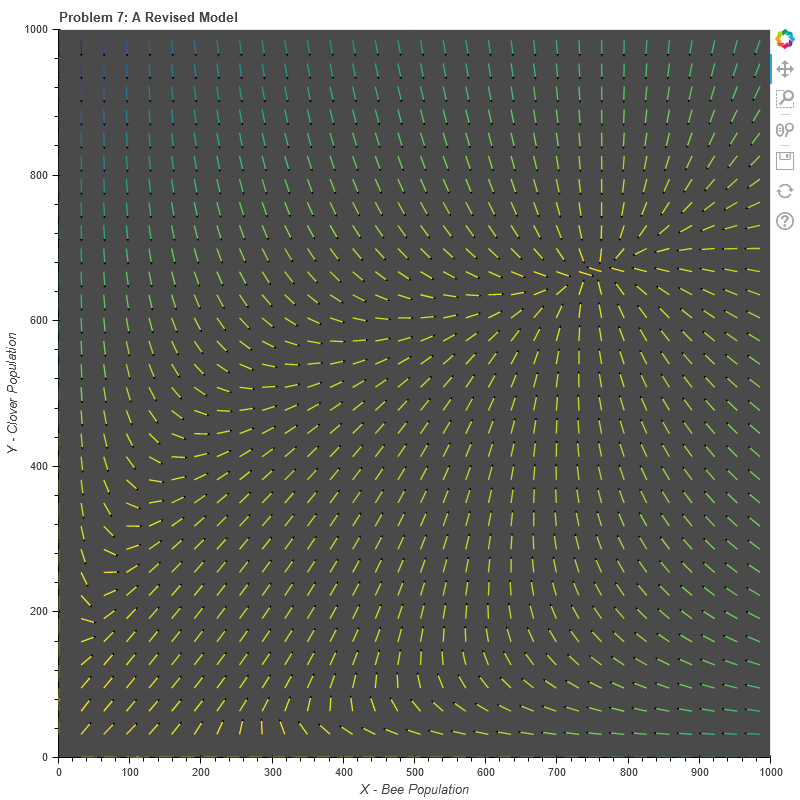
\includegraphics[scale=.5]{charts/problem7_chart.png}}
		\caption{The adjusted model represented as a vector field. It appears that all vectors point towards a path that leads to the stable equilibrium point. }
		\label{fig:p7}
	\end{figure}\\
\end{document}